\documentclass{clic_latex_beamer}

\usepackage{caption}
\usepackage{subcaption}

\begin{document}

\title{Mise en page avancée en \LaTeX}
\author{Quentin Mazars-Simon}
\date{\today}
\institute{École Polytechnique Fédérale de Lausanne}
\titlegraphic{\ccbysa}

\frame{\titlepage}


\begin{frame}
\frametitle{Table des matières}
\tableofcontents[]
\end{frame}

%------------------------------------------
%	Mise en page avancée
%------------------------------------------

\section{Mise en page avancée en \LaTeX}


%-----------------
%	Marges
%-----------------

\subsection{Changer les marges}
\begin{frame}
\frametitle{Changer les marges}
    \begin{itemize}
    \item Les marges par défaut de \LaTeX\ sont un peu trop larges pour certains usages
    \item Il est très facile de les changer avec le package \texttt{geometry} : par exemple \texttt{\textbackslash usepackage[margin=3cm]\{geometry\}} réduit toutes les marges à 3cm.
    \item On peut aussi régler chaque marge individuellement: \texttt{\textbackslash usepackage[left=3cm,right=2cm,top=2cm,bottom=5cm]\\\{geometry\}}.
    \end{itemize}
 \end{frame}
 
 \begin{frame}
\frametitle{Changer les marges: exemples}
\begin{figure}
        \centering
        \begin{subfigure}[b]{0.3\textwidth}
                 \fbox{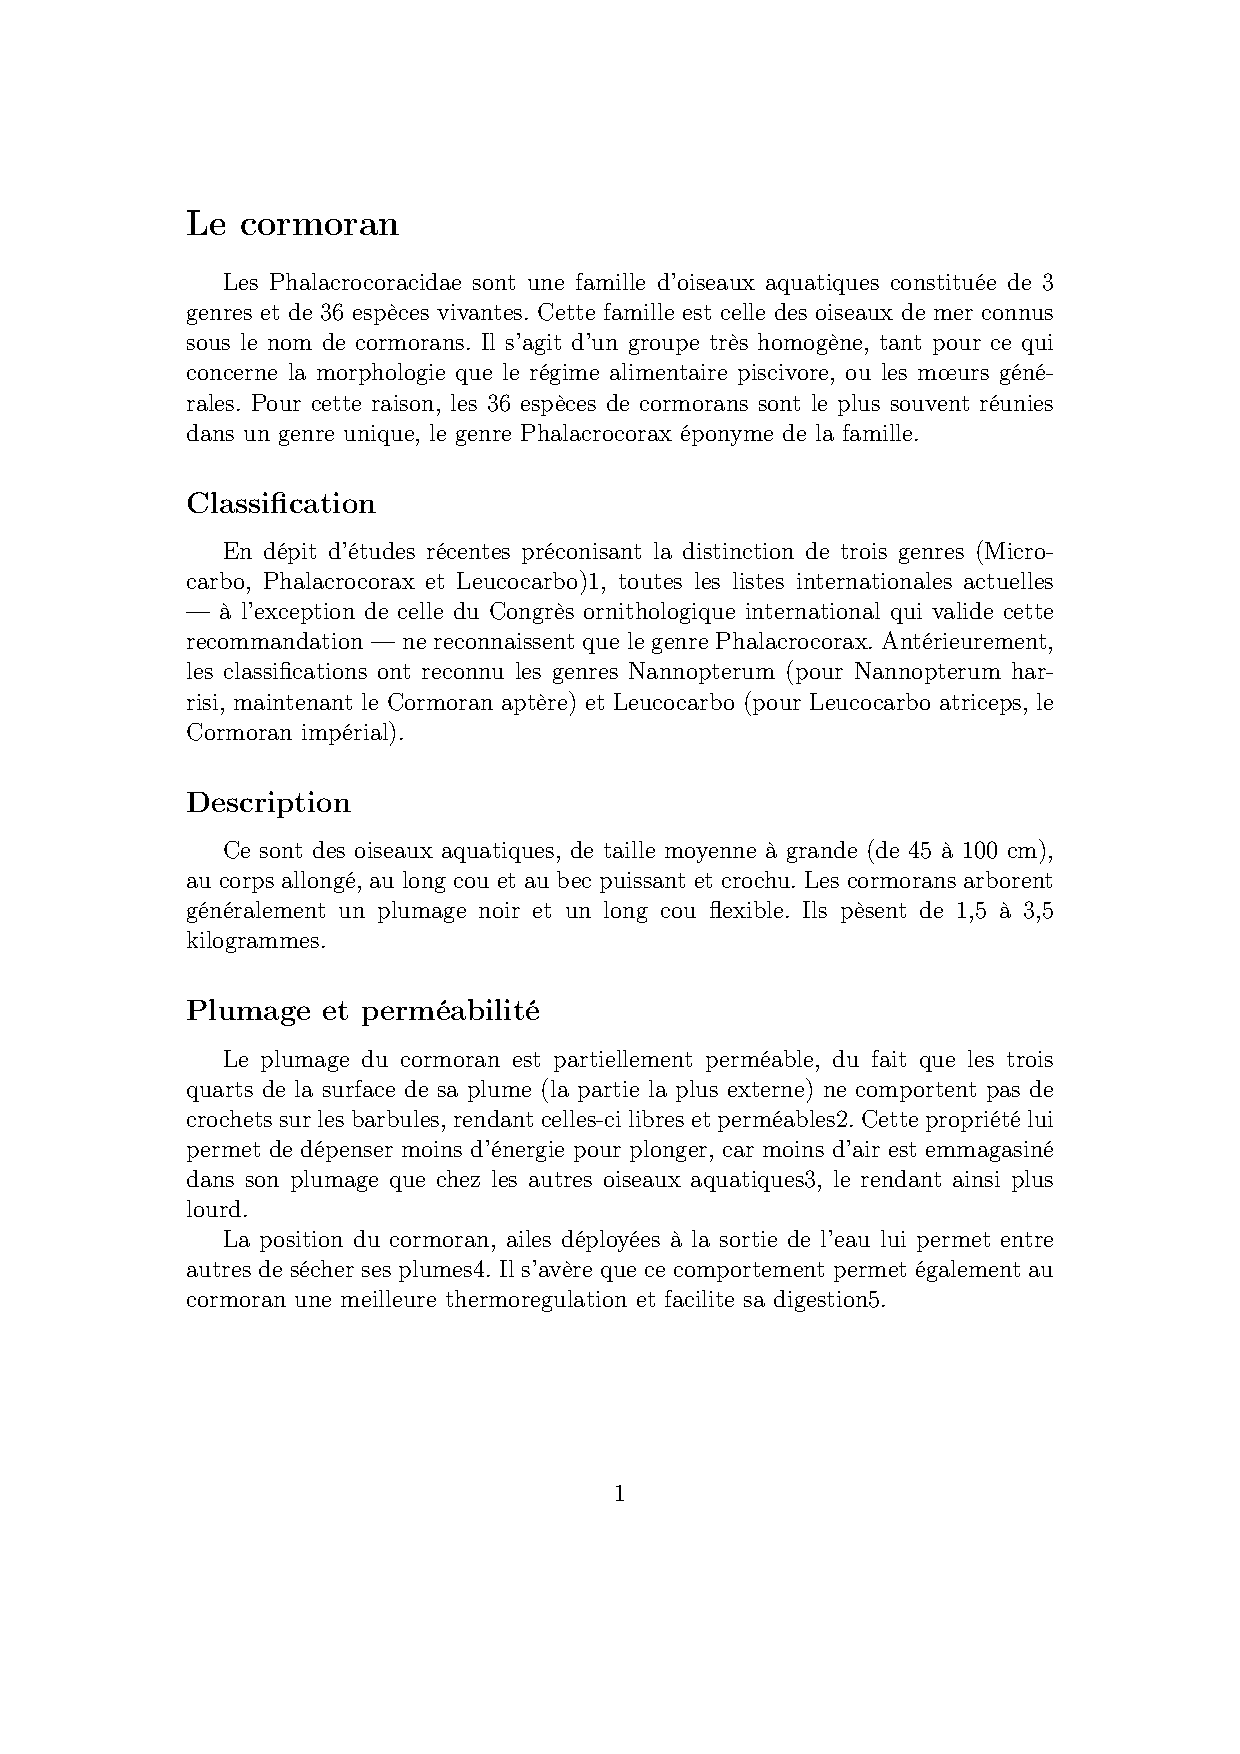
\includegraphics[width=\textwidth]{illustrations/mepa/geometry-default.pdf}}
                \caption*{Par défaut}
        \end{subfigure}
        ~ 
        \begin{subfigure}[b]{0.3\textwidth}
                \fbox{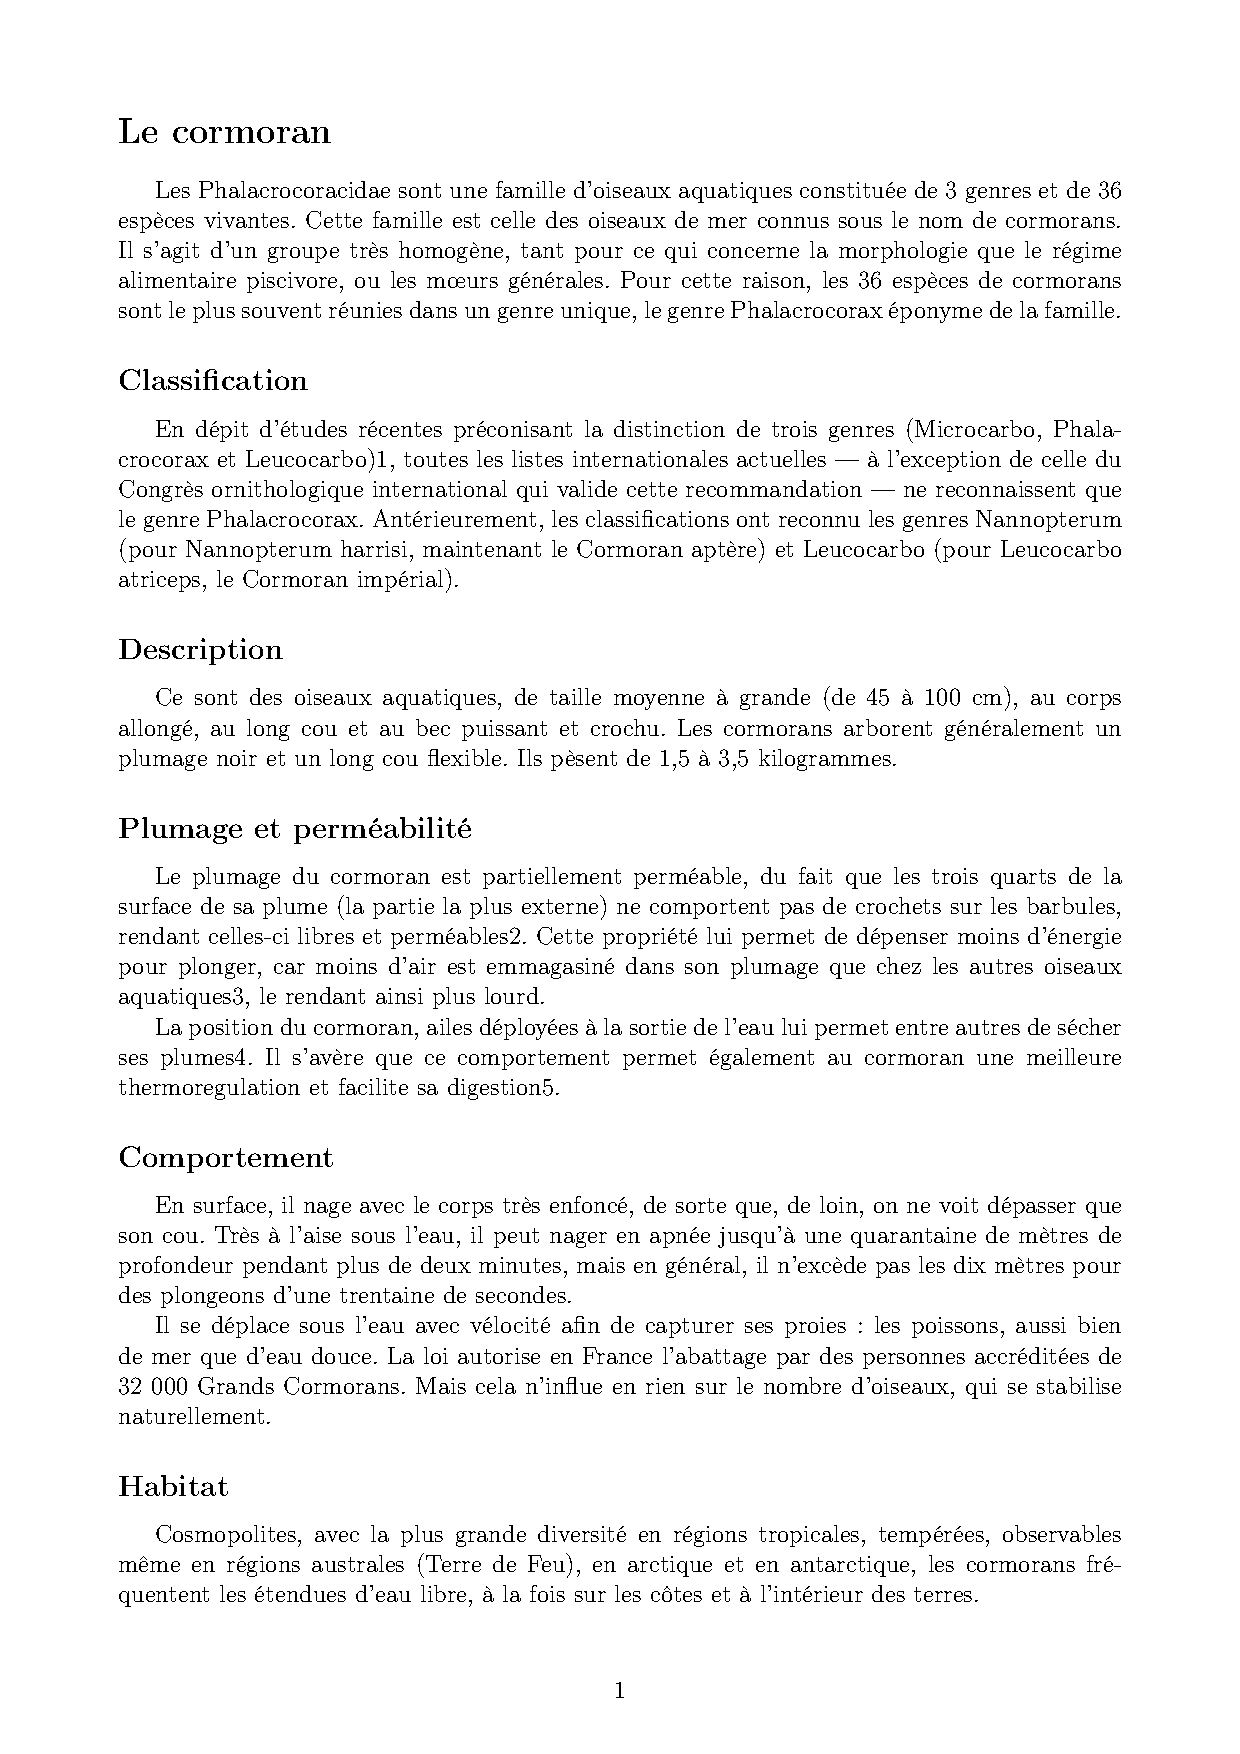
\includegraphics[width=\textwidth]{illustrations/mepa/geometry-2.pdf}}
                \caption*{2cm}
        \end{subfigure}
        ~ 
        \begin{subfigure}[b]{0.3\textwidth}
                \fbox{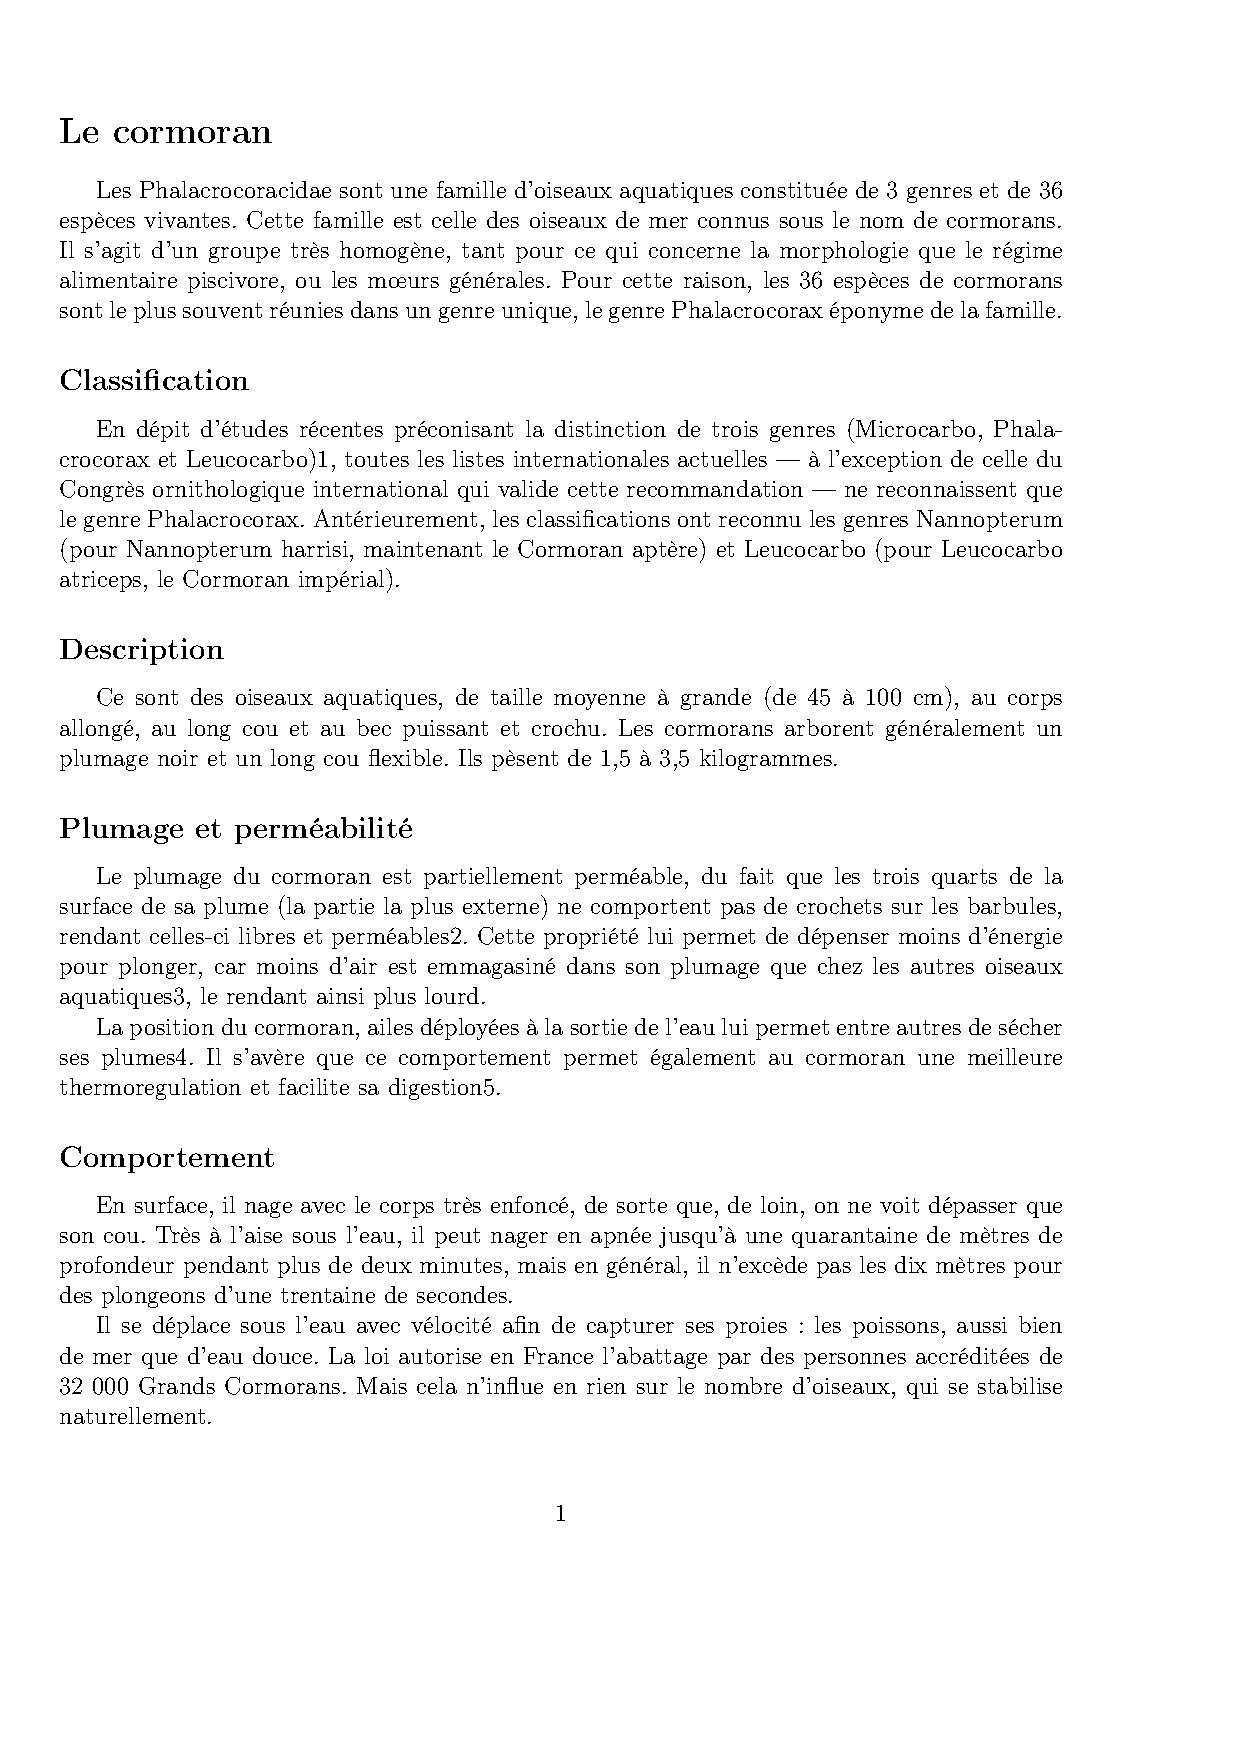
\includegraphics[width=\textwidth]{illustrations/mepa/geometry-13.pdf}}
                \caption*{différentes tailles}
        \end{subfigure}
    \end{figure}
 \end{frame}
 
%----------------------------------------
%	Header & Footer
%----------------------------------------
 
\subsection{Personnaliser les entêtes et pieds de page}
\begin{frame}[fragile]
\frametitle{Personnaliser les entêtes et pieds de page}
    \begin{itemize}
    \item Par défaut les entêtes et pieds de page \LaTeX sont difficiles à personnaliser.
    \item On utilise donc le package \texttt{fancyhdr} qui permet de modifier facilement et de mettre en page les entêtes et pieds de page.
\item Utilisation pour l'entête (respectivement le pied de page):
\begin{lstlisting}
\usepackage{fancyhdr}
...   
\pagestyle{fancy} %Ne pas oublier
\lhead{Ce qui va \\ à gauche} %(\lfoot)
\chead{Ce qui va \\ \textbf{au centre}} %(\cfoot)
\rhead{Ce qui va à droite \\ $E = mc^{2}$} %(\rfoot)
\end{lstlisting}
\end{itemize}
\end{frame}

 
\begin{frame}
\frametitle{Personnaliser entêtes et pieds de page : résultats}
\begin{figure}
        \centering
        \begin{subfigure}[b]{\textwidth}
                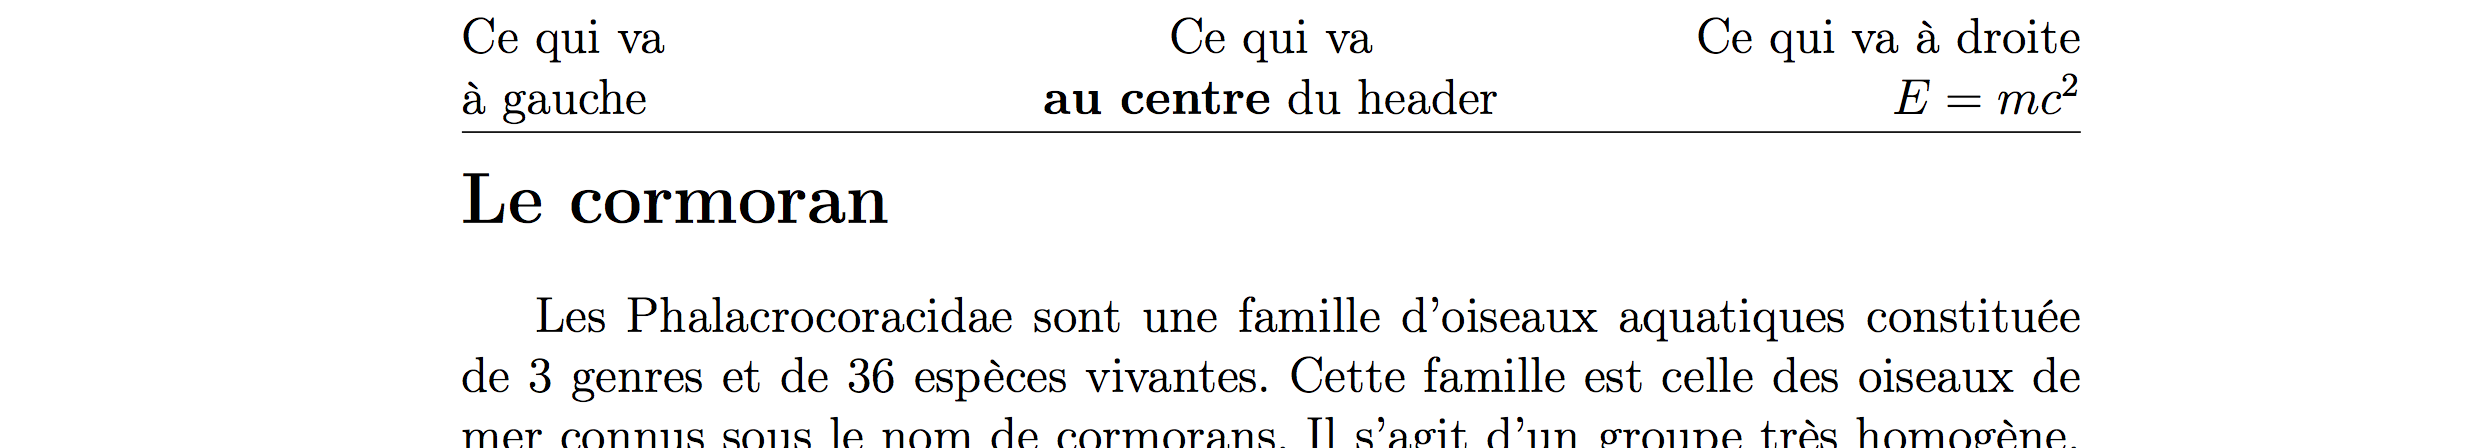
\includegraphics[width=\textwidth]{illustrations/mepa/header.png}
                \caption*{Entête}
        \end{subfigure}
        
        \begin{subfigure}[b]{\textwidth}
              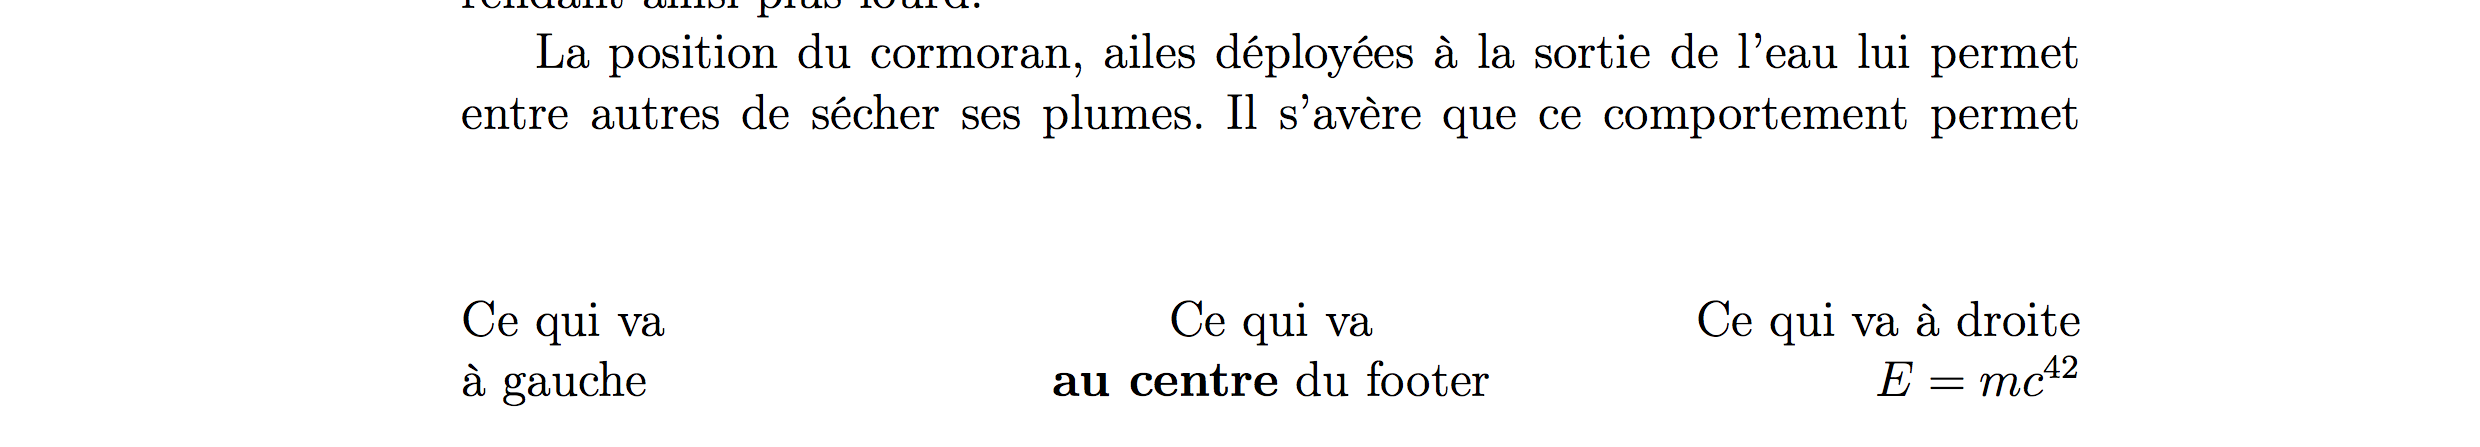
\includegraphics[width=\textwidth]{illustrations/mepa/footer.png}
                \caption*{Pied de page}
        \end{subfigure}
    \end{figure}


\end{frame}

%-------------------------------------
%	Multi-colonnes
%-------------------------------------
 
   \subsection{Créer un document multi-colonnes}
\begin{frame}
\frametitle{Créer un document multi-colonnes}
    \begin{itemize}
    \item Pour certain types de documents (comme les articles scientifique), on veut pouvoir afficher le texte sur plusieurs colonnes.
    \item Pour avoir deux colonnes, il suffit juste d'ajouter un argument à la classe du documents: \texttt{[twocolumn]}: \texttt{\textbackslash documentclass[12pt, twocolumn]\{article\}}
    \item Pour plus de colonnes et/ou plus de flexibilité, il faut utiliser le package \texttt{multicol} qui défini un environnement multicols. Par exemple: \texttt{ \textbackslash begin\{multicols\}\{3\}[intro...]...\textbackslash end\{multicols\}}
    \end{itemize}
 \end{frame}
 

\begin{frame}
\frametitle{Créer un document multi-colonnes: résultats}
\begin{figure}
        \centering
        \begin{subfigure}[b]{0.3\textwidth}
                 \fbox{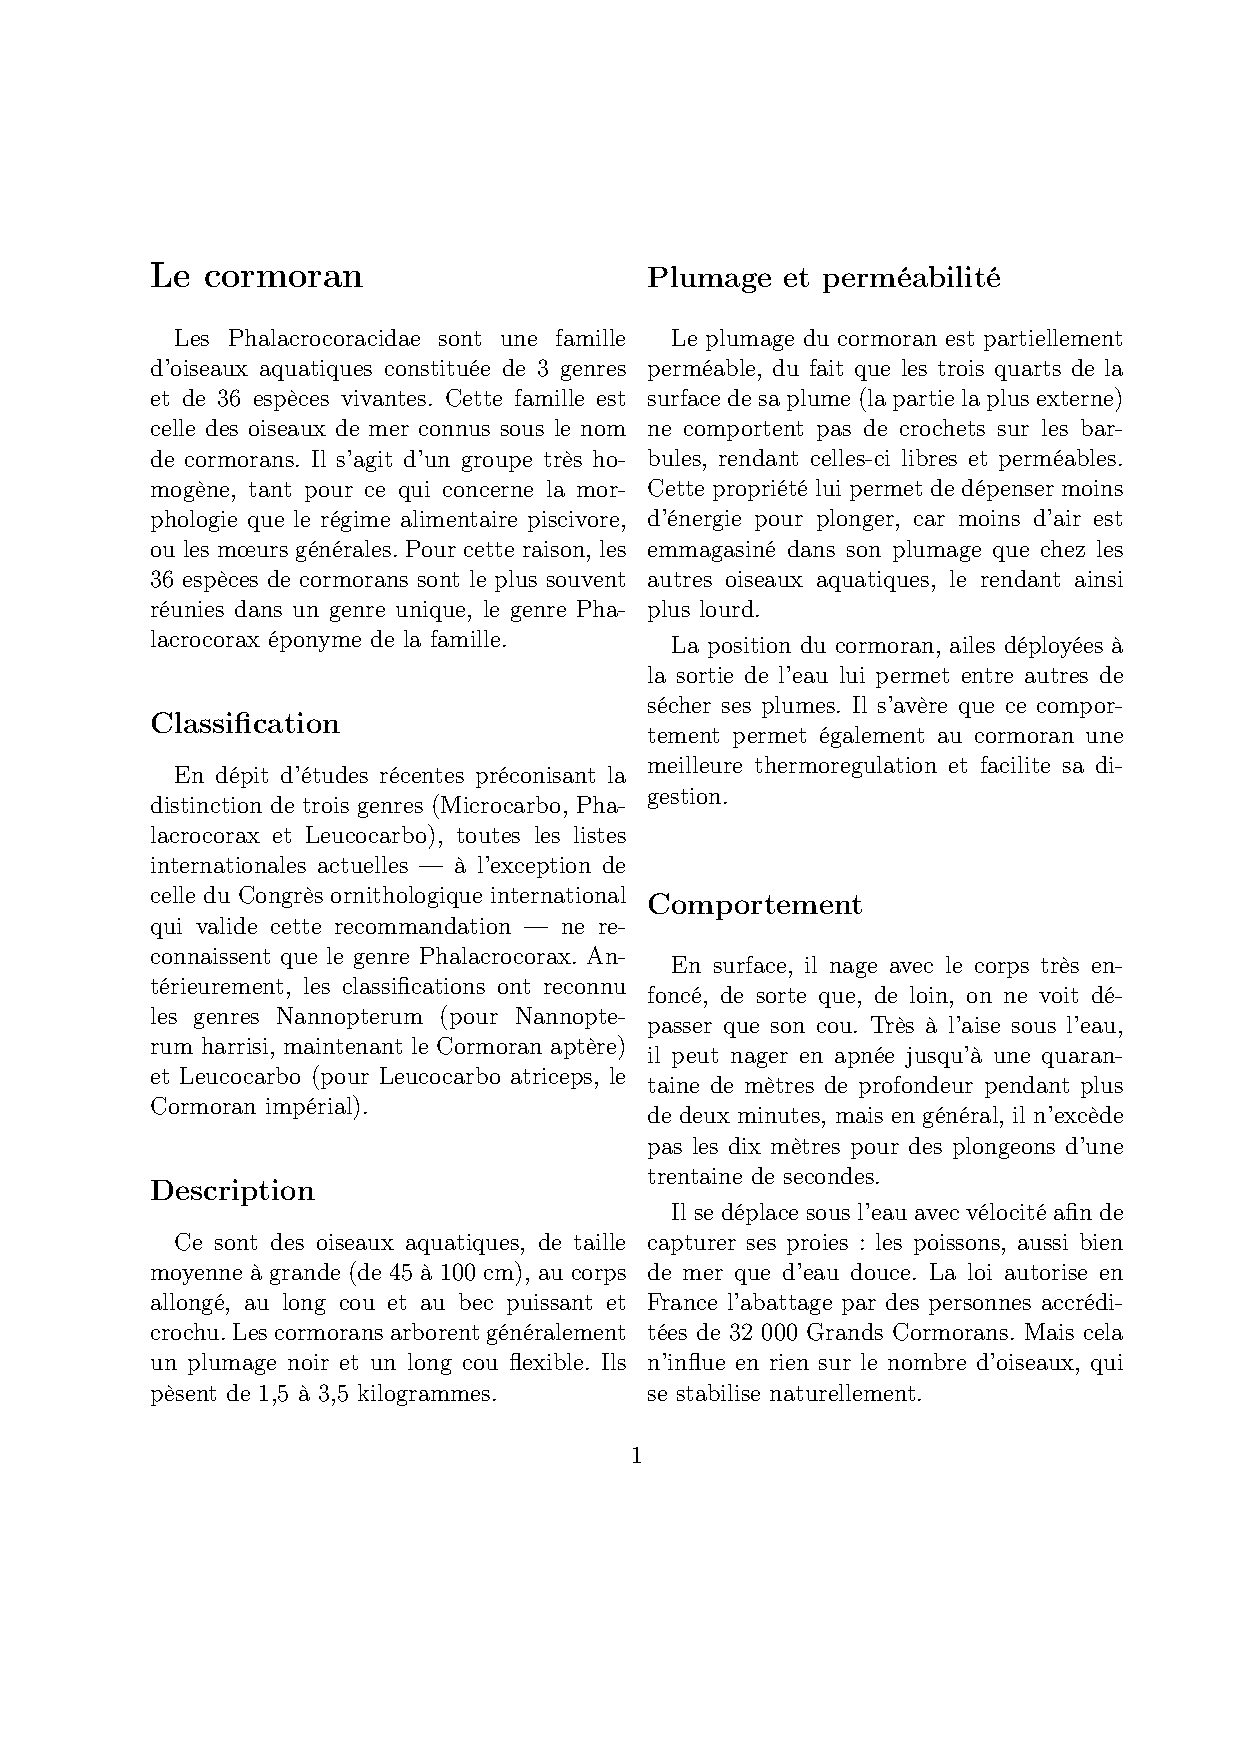
\includegraphics[width=\textwidth]{illustrations/mepa/2cols.pdf}}
                \caption*{2 colonnes}
        \end{subfigure}
        ~ 
        \begin{subfigure}[b]{0.3\textwidth}
                \fbox{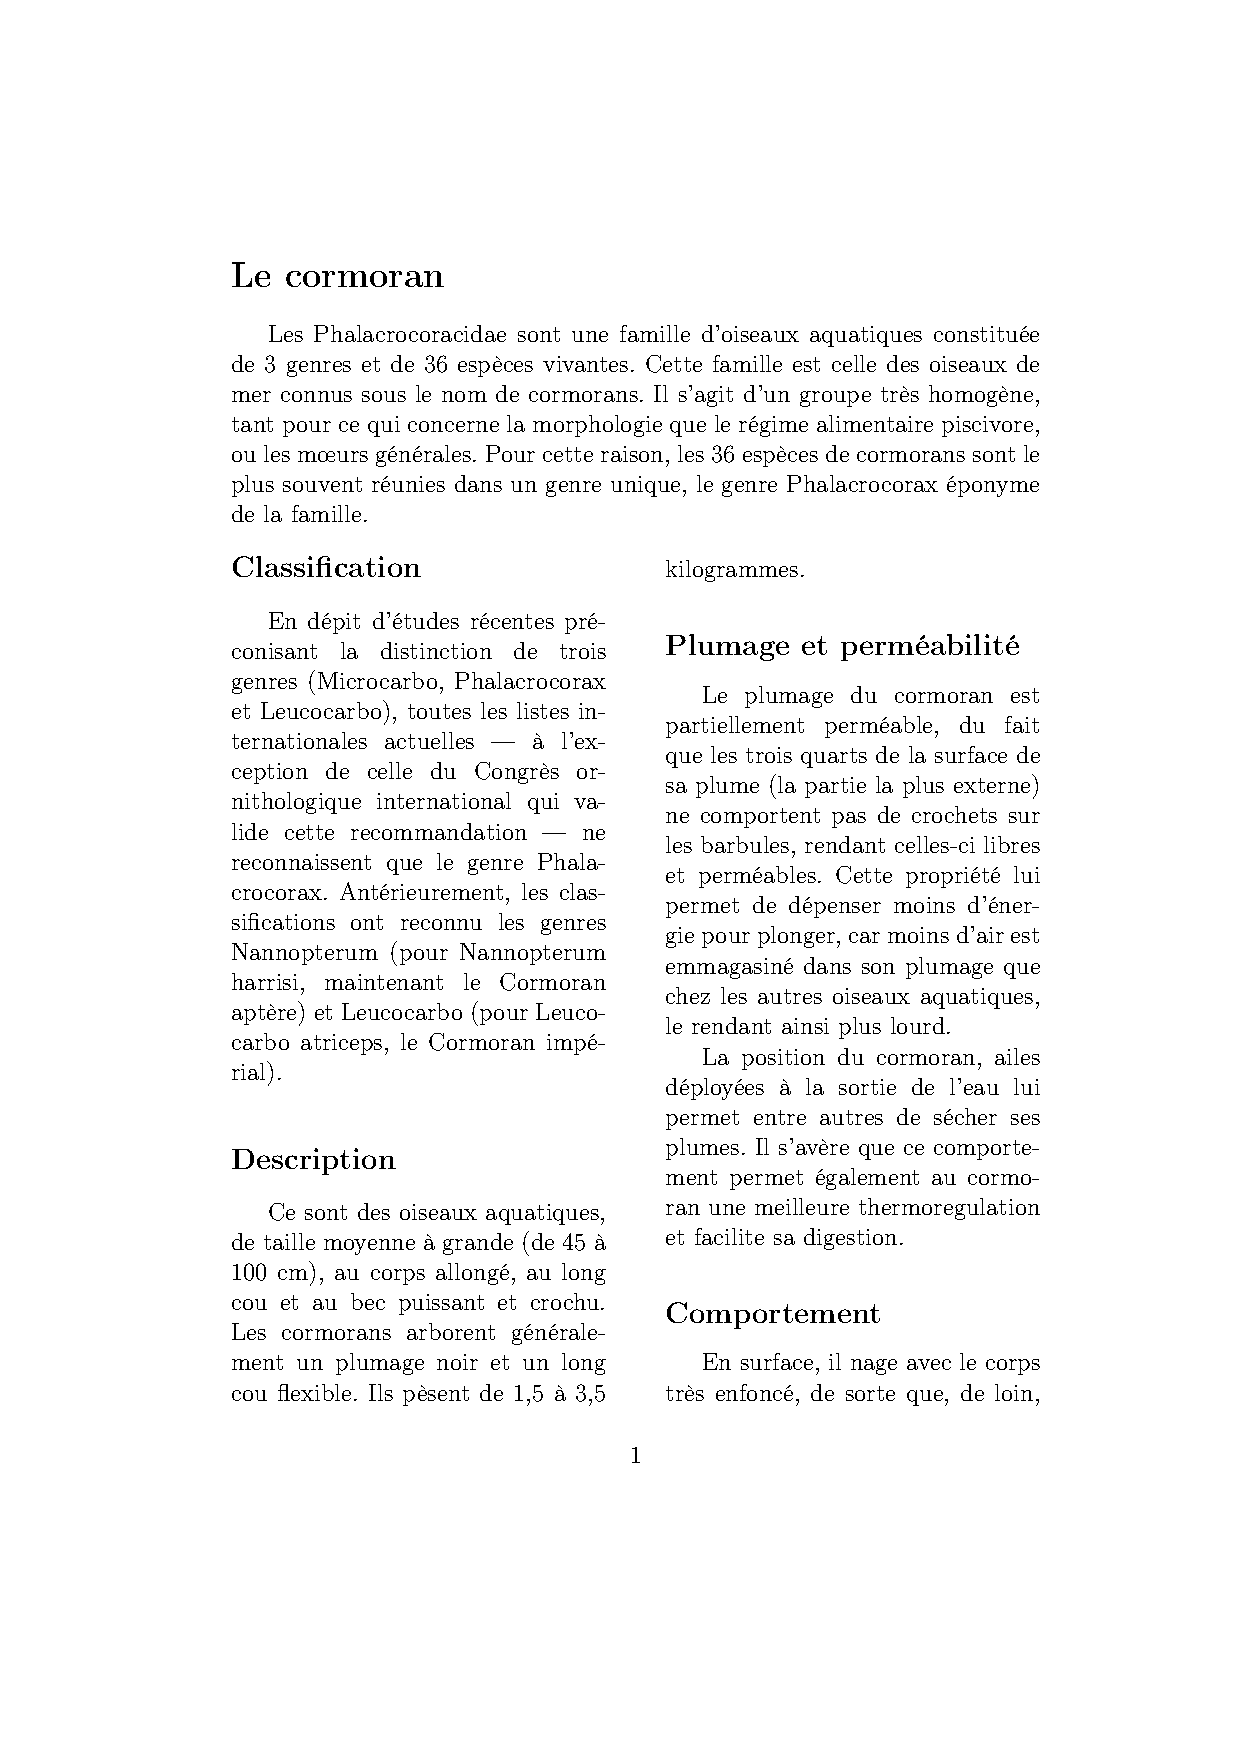
\includegraphics[width=\textwidth]{illustrations/mepa/2cols2.pdf}}
                \caption*{2 colonnes et intro}
        \end{subfigure}
        ~ 
        \begin{subfigure}[b]{0.3\textwidth}
                \fbox{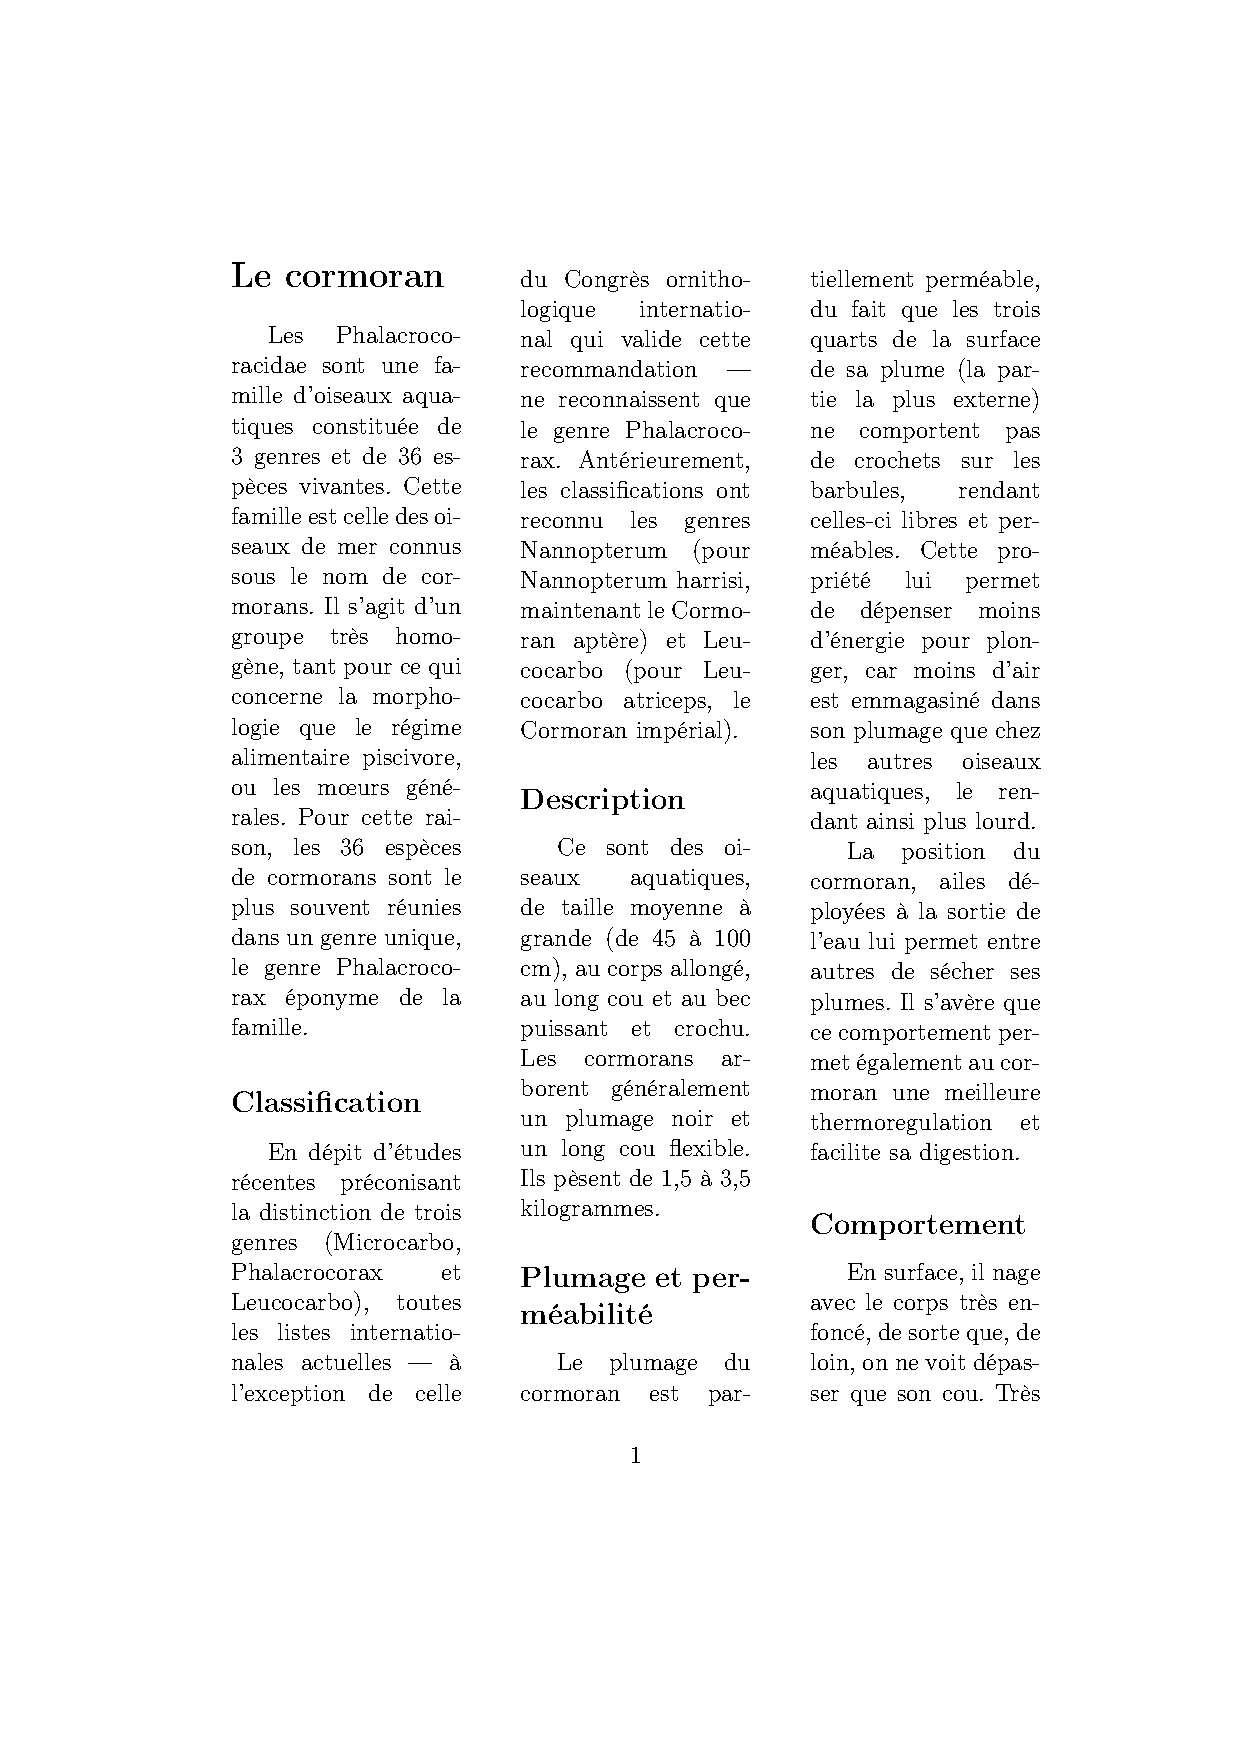
\includegraphics[width=\textwidth]{illustrations/mepa/3cols.pdf}}
                \caption*{3 colonnes}
        \end{subfigure}
    \end{figure}

 \end{frame}
 
 
%------------------------------------------
%	Questions et Références
%------------------------------------------
 
\begin{frame}
\frametitle{Questions ?}
\begin{center}
\Huge Des questions ?
\end{center}
\end{frame}
 
\begin{frame}
\frametitle{Références}
\begin{itemize}
\item \href{https://www.sharelatex.com/learn/Page_size_and_margins}{ShareLaTeX: Page size and margins}
\item \href{https://www.sharelatex.com/learn/Headers_and_footers}{ShareLaTeX: Headers and footers}
\item \href{https://www.sharelatex.com/learn/Multiple_columns}{ShareLaTeX: Multiple columns}
\end{itemize}
\end{frame}


\end{document}
